%--------------------------------------------------------------
% thesis.tex 
%--------------------------------------------------------------
% Corso di Laurea in Informatica 
% http://if.dsi.unifi.it/
% @Facolt\`a di Scienze Matematiche, Fisiche e Naturali
% @Universit\`a degli Studi di Firenze
%--------------------------------------------------------------
% - template for the main file of Informatica@Unifi Thesis 
% - based on Classic Thesis Style Copyright (C) 2008 
%   Andr\'e Miede http://www.miede.de   
%--------------------------------------------------------------
\documentclass[twoside,openright,titlepage,fleqn,
	headinclude,12pt,a4paper,BCOR5mm,footinclude]{scrbook}
%--------------------------------------------------------------
\newcommand{\myItalianTitle}{Integrazione di un prototipo chatbot vocale per pagamenti bancari\xspace}
% use the right myDegree option
\newcommand{\myDegree}{Corso di Laurea Triennale in Informatica\xspace}
\newcommand{\myName}{Gabriele Puliti\xspace}
\newcommand{\myProf}{Lorenzo Bettini\xspace}
\newcommand{\myOtherProf}{Correlatore\xspace}
\newcommand{\mySupervisor}{Tommaso Tamantini\xspace}
\newcommand{\myFaculty}{
	Scuola di Scienze Matematiche, Fisiche e Naturali\xspace}
\newcommand{\myUni}{\protect{
	Universit\`a degli Studi di Firenze}\xspace}
\newcommand{\myLocation}{Firenze\xspace}
\newcommand{\myTime}{Anno Accademico 2018-2019\xspace}
\newcommand{\myVersion}{Version 0.1\xspace}
%--------------------------------------------------------------
\usepackage[italian]{babel}
\usepackage[utf8x]{inputenc}
\usepackage[T1]{fontenc} 
\usepackage[square,numbers]{natbib} 
\usepackage[fleqn]{amsmath}  
\usepackage{ellipsis}
\usepackage{listings}
\usepackage{subfig}
\usepackage{caption}
\usepackage{appendix}
\usepackage{siunitx}
\usepackage{natbib}
\usepackage{listings} %Per inserire codice\usepackage{listings}
\usepackage{color}
\usepackage{graphicx}
\usepackage{wrapfig}
\usepackage{float}
\definecolor{dkgreen}{rgb}{0,0.6,0}
\definecolor{gray}{rgb}{0.5,0.5,0.5}
\definecolor{mauve}{rgb}{0.58,0,0.82}


%--------------------------------------------------------------
\usepackage{dia-classicthesis-ldpkg}
%--------------------------------------------------------------
% Options for classicthesis.sty:
% tocaligned eulerchapternumbers drafting linedheaders 
% listsseparated subfig nochapters beramono eulermath parts 
% minionpro pdfspacing
\usepackage[eulerchapternumbers,linedheaders,subfig,beramono,eulermath,
parts]{classicthesis}
%--------------------------------------------------------------
\newlength{\abcd} % for ab..z string length calculation
% how all the floats will be aligned
\newcommand{\myfloatalign}{\centering} 
\setlength{\extrarowheight}{3pt} % increase table row height
\captionsetup{format=hang,font=small}
%--------------------------------------------------------------
% Layout setting
%--------------------------------------------------------------
\usepackage{geometry}
\geometry{
	a4paper,
	ignoremp,
	bindingoffset = 1cm, 
	textwidth     = 13.5cm,
	textheight    = 21.5cm,
	lmargin       = 3.5cm, % left margin
	tmargin       = 4cm    % top margin 
}

\lstset{
  	frame=tb,
	language=Matlab,
  	aboveskip=3mm,
  	belowskip=3mm,
  	showstringspaces=false,
  	columns=flexible,
  	basicstyle={\small\ttfamily},
  	numbers=none,
  	breaklines=true,
  	breakatwhitespace=true,
  	tabsize=3
}
%--------------------------------------------------------------
\begin{document}
\frenchspacing
\raggedbottom
\pagenumbering{roman}
\pagestyle{plain}
%--------------------------------------------------------------
% Frontmatter
%--------------------------------------------------------------
%--------------------------------------------------------------
% titlepage.tex (use thesis.tex as main file)
%--------------------------------------------------------------
\begin{titlepage}
	\begin{center}
   	\large
      \hfill
      \vfill
      \begingroup
         
\includegraphics[scale=0.15]{logo/LOGO}\\
%			\spacedallcaps{\myUni} \\ 
			\myFaculty \\
			\myDegree \\ 
			\vspace{0.5cm}
         \vspace{0.5cm}    
         Tesi di Laurea    
      \endgroup 
      \vfill 
      \begingroup
      	\color{Maroon}\spacedallcaps{\myItalianTitle} \\ $\ $\\ 	
	\bigskip
      \endgroup
      \spacedlowsmallcaps{\myName}
      \vfill 
      \vfill
      Relatore: \emph{Lorenzo Bettini}\\
      Tutor Aziendale: \emph{Tommaso Tamantini}\\
      \vfill
      \vfill
      \myTime
      \vfill                      
	\end{center}        
\end{titlepage}   
%--------------------------------------------------------------
% back titlepage
%--------------------------------------------------------------
   \newpage
	\thispagestyle{empty}
	\hfill
	\vfill
	\noindent\myName: 
	\textit{\myItalianTitle,} 
	\myDegree, \textcopyright\ \myTime
%--------------------------------------------------------------
% back titlepage end
%--------------------------------------------------------------
\pagestyle{scrheadings}
%--------------------------------------------------------------
% Mainmatter
%--------------------------------------------------------------
\pagenumbering{arabic}
% use \cleardoublepage here to avoid problems with pdfbookmark
%\include{intro} % use \myChapter command instead of \chapter
\tableofcontents
%\listoffigures
\cleardoublepage
\thispagestyle{empty}
\begin{flushright}
\null\vspace{\stretch {1}}
\emph{"Se puoi farlo te allora lo pu\`{o} fare anche lei" \break --- Me stesso} \vspace{\stretch{2}}\null
\end{flushright}
\chapter{Introduzione}
\section{Azienda e Software BPS}
Al giorno d'oggi l'utilizzo della voce per automatizzare i processi della vita quotidiana si sta sempre più espandendo, dall'assistente vocale nella propria casa a quello nel proprio cellulare. Sono sempre stato incuriosito da queste tecnologie e il tirocinio era il modo migliore per comprendere lo sviluppo di software di questo tipo. Il progetto mi è stato proposto dall'azienda fiorentina E.D.P. Service, società collegata al gruppo Best Vision Holding, il cui scopo era integrare una funzionalità nuova nel sito del cliente BPS(suisse) che permettesse di eseguire pagamenti o trasferimenti di denaro usando linguaggio naturale comunicando direttamente con l'applicazione.
\section{Analisi del problema}
Il software su cui avrei dovuto lavorare era una classica web application di monetica \footnote{La monetica è l'insieme delle tecniche di pagamento attraverso strumenti informatici e telematici}. Software di questo tipo si suddividono in 2 parti: una parte adibita all'interazione utente definita interfaccia grafica o frontend e la parte che gestisce le informazioni chiamata backend o lato server.
La parte del frontend gestisce principalmente le modalità di accesso dell'utente consentendogli di interagire con l'applicativo eseguendo le azioni messe a disposizione, come ad esempio: visualizzare il numero di transazioni eseguite, creare un pagamento, controllare l'andamento del mercato in base a una determinata valuta.
Per riuscire a sviluppare un'integrazione in questo sistema ho studiato i linguaggi usati dalla piattaforma della banca, principalmente formata da codice HTML, CSS, e AngularJS.
L'ultimo citato è un web-framework di casa Google scritto in JavaScript che permette di dinamicizzare una pagina web utilizzando dei comandi a livello di codice HTML, chiamati direttive, che vengono poi eseguiti da AngularJs una volta che la pagina web viene caricata dal browser.
Tutto ciò che riguarda il lato server: gestione, elaborazione e immagazzinamento dei dati forniti dal frontend viene eseguita dal backend, parte fondamentale di un servizio web bancario che deve garantire sicurezza e reperibilità dei dati. Il backend sviluppato da Best Vision è diviso in un servizio di database e uno di gestione del database scritto per intero in linguaggio Java usando il framework Spring.
I pagamenti compiuti tramite la piattaforma web utilizzano la classica procedura di compilamento manuale di alcuni campi di testo, come ad esempio la quantità di denaro da trasferire e l'iban del conto del destinatario.
Inserire una funzionalità che permettesse di eseguire queste azioni usando la sola voce avrebbe diminuito il numero di azioni che l'utente avrebbe dovuto eseguire per ottenere ciò che cercava, dovevo quindi imitare il comportamento umano di un operatore di banca. Per fare questo è stato pensato di sviluppare un servizio di chat bot che riuscisse a comprendere il linguaggio naturale umano e producesse una risposta in completa autonomia eseguendo le azioni necessarie richieste dall'utente.
Il pagamento tramite chat doveva quindi eseguire tutte le richieste al server nel giusto ordine prima di completare la transazione voluta: autorizzazione per accedere al conto dell'utente, richiesta di trasferimento di capitale verso terzi e delega della conferma del transazione.
Nel mio caso il frontend è rappresentato dalla chat in cui l'utente può decidere se scrivere un testo con linguaggio naturale oppure utilizzare il servizio vocale, il backend invece è composto da un'intelligenza artificiale che genera una risposta e agisce in base alle richieste.
Quando un utente invia un messaggio si aspetta che venga generata una risposta consona, cioè venga eseguita una analisi del testo e che venga formulata una frase di senso compiuto che riesca a rispondere in maniera corretta al messaggio inviato.
L'analisi del testo viene definita comprensione del linguaggio naturale, in inglese Natural Language Understanding (NLU), cioè attribuire alla frase analizzata un intento ed estrarre da essa oggetti che possono essere utili per la generazione di una risposta.
L'effettiva generazione della risposta però non è un compito che viene esercitato dal NLU, ma da un Natural Language Generator (NLG) che in base all'analisi precedente riesca a determinare la miglior risposta possibile.
\begin{figure}[H]
 \centering
    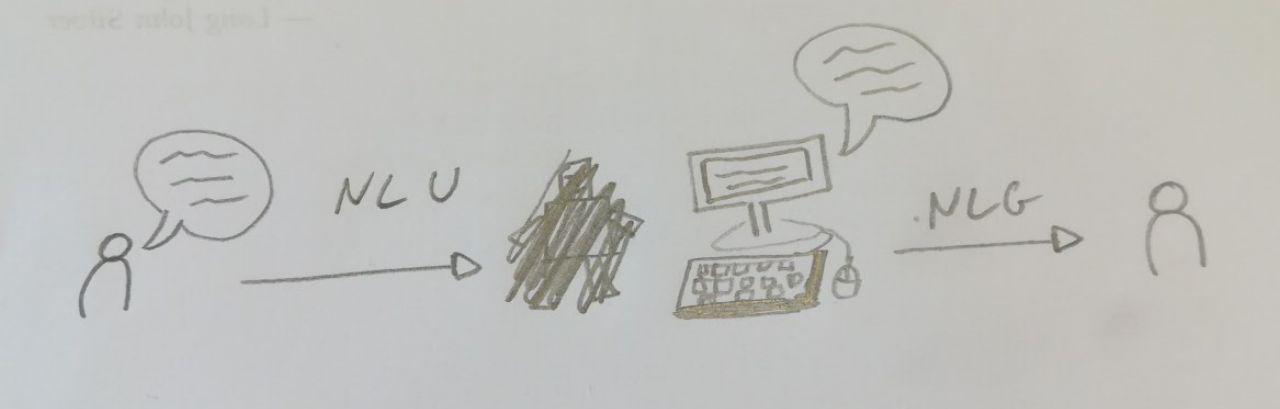
\includegraphics[width=0.4\textwidth]{img/nlu_nlg.jpg}
 \caption{Nlu and Nlg}
\end{figure}
\section{Sviluppo del chatbot}
Il chatbot voluto è quindi formato dalla chat e 2 tipi di intelligenza artificiale: una che esegue il NLU e un'altra che racchiuda il compito di NLG.
\iffalse
https://en.wikipedia.org/wiki/Natural-language_understanding
https://www.expertsystem.com/natural-language-understanding-different-nlp/
https://rasa.com/
https://rasa.com/docs/get\_started\_step1/
https://www.techopedia.com/definition/33013/natural-language-understanding-nlu
https://www.sisense.com/glossary/natural-language-understanding/
\fi
Per la creazione del bot ho usato una libreria open source sviluppata in Python chiamata \textbf{Rasa}, che mette a disposizione tutti gli strumenti che servono per poter sviluppare intelligenze artificiali di questo tipo. I tools che ho usato sono: rasa\_nlu e rasa\_core, il primo per eseguire il compito di NLU e l'altro quello di NLG eseguendo anche le azioni necessarie.
La corretta esecuzione degli strumenti appena descritti si basa su modelli generati grazie a dataset precedentemente realizzati, i quali contengono veri e propri esempi di frasi e possibili conversazioni che l'utente potrebbe usare.
Teoricamente questo tipo di processo richiederebbe un numero molto elevato di esempi per essere più preciso, in questo caso però mi è bastato creare un dataset con una popolazione di soli 60 esempi per ottenere un prototipo di bot ragionevolmente preciso.
Completato lo sviluppo delle 2 intelligenze artificiali queste sono state collocate in un server dove potessero rimanere in ascolto di tutti i messaggi da parte dei clienti.
L'ultimo passo è stato quello di integrare il prototipo della chat nel sito web di BPS(suisse) attuando alcune modifiche sia lato backend, in cui sono state aggiunte alcune proprietà per rendere il server più sicuro, sia lato frontend, modificando la web application includendo la chat da me creata.
Questo ha completato il lavoro di tirocinio consentendo all'azienda di inserire nella fase di produzione e miglioramento l'integrazione da me sviluppata.
\begin{figure}[H]
 \centering
    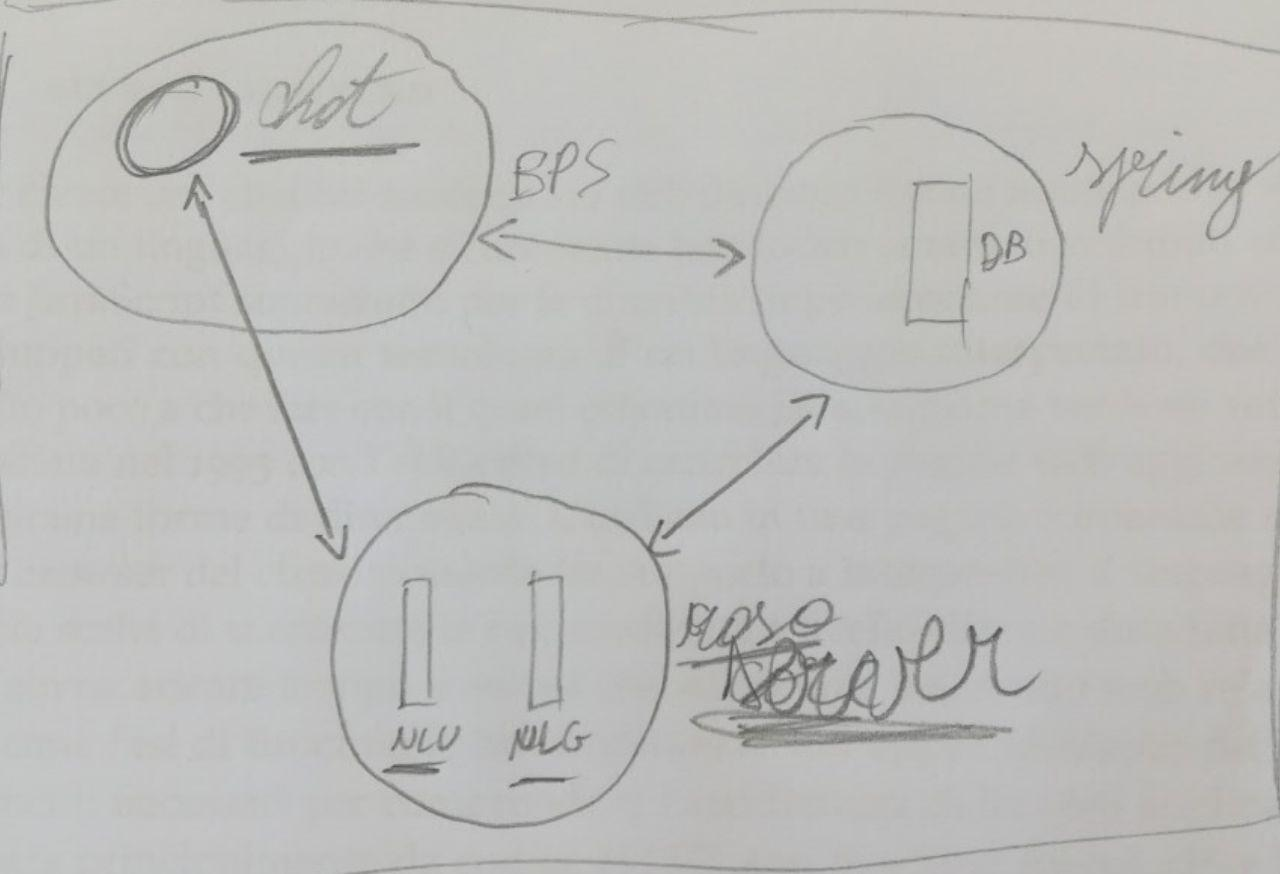
\includegraphics[width=0.4\textwidth]{img/last_architecture.jpg}
 \caption{Architecture}
\end{figure}

\iffalse
I pagamenti compiuti tramite la piattaforma web utilizzano la classica procedura di compilamento manuale di alcuni campi di testo, come ad esempio la quantità di denaro da trasferire e l'iban del conto del destinatario.
\fi

\chapter{Pre-integrazione}


\section{Studio frontend}
\iffalse
<studio di javascript>
\fi
Per creare una chat nei moderni siti web dinamici \'e stato necessario lo studio di un linguaggio che sicuramente ha modernizzato lo sviluppo web cio\'e JavaScript soprattutto per la quantit\'a impressionante di framework sviluppati con questa tecnologia.
\'E un linguaggio interpretato, che ha molto poco a che fare con il quasi omonimo Java, la prima versione venne rilasciata nel 1995 con l'obbiettivo di arricchire le pagine web aggiungendo alcune forme di dinamicit\'a. L'utilizzo in una pagina \'e possibile solo se il browser del client possiede un supporto a interpretare il linguaggio, questa scelta di mantenere la responsabilit\'a a livello client \'e stata fatta per non sovracaricare troppo il server che riliasciava il servizio web relativo.
\iffalse 
<studio di angularjs nel libro (vedi https://github.com/Wabri/UniversityInternship#day-01-020518--55-ore)>
\fi
Le prime fasi di tirocinio le ho concentrate sull'apprendimento dei vari strumenti necessari per comprendere l'architettura della web application formata principalmente da codice HTML con direttive AngularJS e Javascript, tenuti insieme dal MVC (Model View Controller).
Il MVC \'e un pattern architetturale basato su 3 componenti che hanno lo scopo di usare e gestire i dati con scopi differenti: il model deve gestire i dati e fornire metodi per usarli nonch\'e la logica e le regole dell'applicazione, il view ha lo scopo di rappresentare i dati sotto forma di informazione in modo tale da interagire con l'utente che li visualizzer\'a, e infine il controller che attraverso istruzioni fornite dall'utente modifica lo stato degli altri 2 componenti modificando i dati gestiti dal controller o indicando una modalit\'a differente di visualizzazione dei dati al view.
\begin{figure}[H]
 \centering
  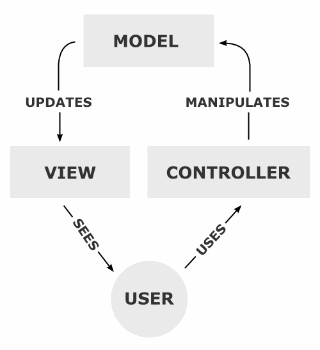
\includegraphics[width=0.3\textwidth]{img/MVC-Process.png}
 \caption{MVC}
 \end{figure}
Questa struttura viene usata principalmente per dividere la logica di business, che \'e la parte di eleborazione dati, con l'interfaccia utente, migliorando quindi l'organizzazione dei processi interni di una application. 
L'utilizzo di questo pattern direttamente sul client ha permesso un cambiamento importante per quanto riguarda le dynamic pages, cio\'e quello di non eseguire un redirect per modificare la pagina ma eseguendo chiamate asincrone al server. 
Con il tempo \'e stato necessario fornire un framework che implementasse queste logiche riducendo i tempi di sviluppo andando a generalizzare tutti quei comportamenti classici del pattern MVC, se si parla di JavaScript senza alcun dubbio il framework pi\'u usato \'e AngularJs.
Questa libreria funziona per mezzo di comandi, definiti direttive, che vengono inserite direttamente nel codice HTML che permettono di eseguire una sorta di comunicazione tra le varie parti del client. Il framework viene caricato all'interno della pagina attraverso l'import definito dal tag <script> in questo modo:
\lstset{ 
  backgroundcolor=\color{white},   % choose the background color; you must add \usepackage{color} or \usepackage{xcolor}; should come as last argument
  basicstyle=\footnotesize,        % the size of the fonts that are used for the code
  breakatwhitespace=false,         % sets if automatic breaks should only happen at whitespace
  breaklines=true,                 % sets automatic line breaking
  captionpos=b,                    % sets the caption-position to bottom
  commentstyle=\color{green},    % comment style
  deletekeywords={...},            % if you want to delete keywords from the given language
  escapeinside={\%*}{*)},          % if you want to add LaTeX within your code
  extendedchars=true,              % lets you use non-ASCII characters; for 8-bits encodings only, does not work with UTF-8
  firstnumber=0,                % start line enumeration with line 1000
  frame=single,	                   % adds a frame around the code
  keepspaces=true,                 % keeps spaces in text, useful for keeping indentation of code (possibly needs columns=flexible)
  keywordstyle=\color{blue},       % keyword style
  language=HTML,                 % the language of the code
  morekeywords={*,...},            % if you want to add more keywords to the set
  numbers=none,                    % where to put the line-numbers; possible values are (none, left, right)
  numbersep=5pt,                   % how far the line-numbers are from the code
  numberstyle=\tiny\color{gray}, % the style that is used for the line-numbers
  rulecolor=\color{black},         % if not set, the frame-color may be changed on line-breaks within not-black text (e.g. comments (green here))
  showspaces=false,                % show spaces everywhere adding particular underscores; it overrides 'showstringspaces'
  showstringspaces=false,          % underline spaces within strings only
  showtabs=false,                  % show tabs within strings adding particular underscores
  stepnumber=2,                    % the step between two line-numbers. If it's 1, each line will be numbered
  stringstyle=\color{mauve},     % string literal style
  tabsize=3,	                   % sets default tabsize to 2 spaces
  title=\lstname                   % show the filename of files included with \lstinputlisting; also try caption instead of title
}
\begin{lstlisting}
<script 
 src="https://ajax.googleapis.com/ajax/libs/angularjs/1.2.19/angular.js">
</script>
\end{lstlisting}
Questo script esegue una lettura dell'intera pagina dove saranno presenti le direttive che dovr\'a eseguire che modificheranno (o no) le sezioni che vogliamo essere dinamiche della pagina.

\section{Creazione della chat stand alone}
Apprese le conoscenze base di questi strumenti ho cominciato con la stesura di una prima versione della chat testuale stand alone in JavaScript. Una chat presuppone la comunicazione tra pi\'u di 2 soggetti, nel mio caso un soggetto \'e rappresentato da l'utente della banca che usa la chat e l'altro il bot, una comunicazione di questo tipo è possibile implementarla usando i sockets.
I sockets sono la soluzione migliore per chat real-time che prevedouno una communicazione bidirezionale tra un client e server, questo prevede quindi che un client mandi un messaggio in chat e il server prende l'incarico di ridirezionare il messaggio al destinatario effettivo. Un socket rimane attivo in ascolto in un canale di comunicazione permettendo lo scambio in input e output di messaggi, in base al tipo di messaggio il socket eseguir\'a una azione specifica che nel caso di una chat \'e stampare o inviare un messaggio. Per fare questo ho usato una libreria JavaScript chiamata socket.io (https://socket.io) che tramite il metodo emit permette di emettere un messaggio in output:
\lstdefinelanguage{JavaScript}{
  keywords={typeof, new, true, false, catch, function, return, null, catch, switch, var, if, in, while, do, else, case, break},
  keywordstyle=\color{blue}\bfseries,
  ndkeywords={class, export, boolean, throw, implements, import, this},
  ndkeywordstyle=\color{darkgray}\bfseries,
  identifierstyle=\color{black},
  sensitive=false,
  comment=[l]{//},
  morecomment=[s]{/*}{*/},
  commentstyle=\color{purple}\ttfamily,
  stringstyle=\color{red}\ttfamily,
  morestring=[b]',
  morestring=[b]"
}
\lstset{
   language=JavaScript,
   backgroundcolor=\color{white},
   extendedchars=true,
   basicstyle=\footnotesize\ttfamily,
   showstringspaces=false,
   showspaces=false,
   numbers=left,
   numberstyle=\footnotesize,
   numbersep=9pt,
   tabsize=2,
   breaklines=true,
   showtabs=false,
   captionpos=b
}
\begin{lstlisting}
// inviare un messaggio
socket.emit('text message', text);
\end{lstlisting} 
Una volta che il messaggio viene emesso un altro socket deve ricevere questo messaggio, \'e quindi necessario che il socket del controller sia sempre in ascolto di messaggi e in base al tipo del messaggio esegua una determinata azione:
\begin{lstlisting}
// connessione e gestione del messaggio
const io = require('socket.io')(server);
io.on('connection', function (socket) {
    socket.on('text message', (text) => {
        // gestione del messaggio
    });
});
\end{lstlisting}
Uno dei motivi principali dello sviluppo di un chatbot \'e quello di permettere all'utente di parlare direttamente al bot usando la voce. Per fare questo ho dovuto usare uno strumento che trasformasse la voce catturata dal microfono in un testo, per la precisione in una stringa da poter inviare tramite il socket al server, un tool di questo tipo \'e definito speech recognition, in italiano riconoscimento vocale.
Ho usato una libreria sviluppata da mozilla chiamata proprio SpeechRecognition (https://developer.mozilla.org/en-US/docs/Web/API/SpeechRecognition) che impostando semplicemente la lingua mi ha permesso di trasformare il parlato dell'utente in una stringa utilizzabile all'interno del client. 
Nel codice HTML ho inserito semplicemente un bottone che attiva il microfono e abilita la funzione di speech recognition
\iffalse
mettere codice? oppure continuare la spiegazione
\fi
Una volta implementata la comunicazione dei messaggi della chat, dato una voce al bot e infine messo a punto una grafica base (vedi figura 2) con dei pulsanti, una casella di testo in cui l'utente potesse scrivere e una zona in cui venissero stampati gli ultimi messaggi scambiati:
\begin{figure}[H]
 \centering
  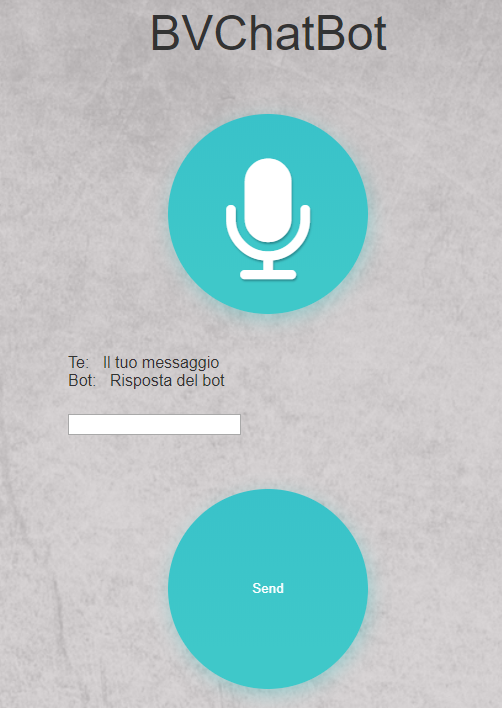
\includegraphics[width=0.4\textwidth]{img/prototype.png}
 \caption{Chat prototype}
 \end{figure}

\section{Creazione dell'intelligenza artificiale}

\subsection{Google-Dialogflow}

\subsection{Rasa}

\subsection{Creazione data set per training}

\section{Aggiornamento Frontend per la comunicazione con Rasa}

\section{Sistema di pagamento vocale}

\section{Funzionamento e esecuzione}

\iffalse
<creazione di una chat testuale>
<integrazione di un sistema di speech recognition>
<inserimento della comunicazione tra la chat e dialogflow>
<vari test di funzionamento della comunicazione>
<passaggio da dialogflow a rasa>
<studio di rasa nlu>
<creazione di un primo modello di training con vari esempi esterni al progetto>
<processo di apprendimento del funzionamento effettivo di rasa lungo>
<tentativo di utilizzo del modello creato precedentemente, con dialogflow, per la creazione del modello di rasa nlu>
<passaggio di competenze(?) da dialogflow a rasa, eliminando la comunicazione effettiva con google>
<connessione con il server bps e rasa>
<per errore ho lasciato che la chat inviasse ancora i dati di test ai server di dialogflow = rasa>dialogflow>
<tutor universitario consiglia l'uso di typescript => studio di typescript => riscrittura della chat usando typescript>
<typescript migliore lettura del codice e possibilità di creazione di classi e oggetti>
<estrapolazione dei dati utente dal server della banca usando chiamate rest>
<generazione data set dell'intelligenza artificiale>
<necessario un server che eseguisse azioni richieste>
<studiare python per poter creare esempi di rasa core>
<studio di rasa core - server>
<utilizzo di chiamate rest all'interno del chatbot verso rasa core>
<problemi con la messa in opera del server su macchina windows>
<utilizzo del server su rete locale per i test>
<refactor del codice chatbot usando superagent (vedi https://github.com/Wabri/UniversityInternship#day-26-110718--55-ore)>
<iniziato a creare le story per generare un modello efficace di intelligenza>
<Cominciato a generare le prime azioni di risposta in base agli intenti e al contenuto del testo fornito in input>
<Creato l'effettivo bot scritto in python, dove risiedono tutte le azioni che può fare il bot>
<Migliorato il modello di training aggiungendo nuovi esempi di intents e stories>
<problemi con l'autenticazione a 2 fattori per il prototipo, non riesce a estrarre direttamente user e password e devo inserirle manualmente con chiamate post verso il server rasa>
<completamento comunicazione user-rasafrontend-rasabackend-backendspringbanca - vedi https://github.com/Wabri/UniversityInternship/blob/master/README.md#day-36-020818--65-ore>
<creazione delle azioni effettive che deve fare il bot rasa backend>
<il problema del xcsrf token e jsession>
<vedi https://github.com/Wabri/UniversityInternship/blob/master/README.md#day-38-210818--75-ore per maggiori informazioni>
<documentazione prototipo>
\fi
\chapter{Integrazione}

\section{Struttura del software internet banking BPS}

\subsection{AngularJs}

\subsection{Spring}

\section{Collegamento chat stand alone con servizi server spring}

\section{Aggiornamento sistema di pagamenti vocali}

\section{Integrazione definitiva nel software aziendale}

\section{Differenze di esecuzione nella nuova piattaforma}

\section{Il problema del jsession token}

\iffalse
<inizio integrazione del prototipo, vedi: https://github.com/Wabri/UniversityInternship/blob/master/README.md\#day-41-280818--7-ore>
<trasformazione delle librerie usate nel prototipo con strumenti angularjs>
<refactor del prototipo>
<speech recognition in angularjs>
<synth voice in angularjs>
<creazione del server rasa su server aziendale>
<creazione della documentazione nella wiki best vision>
<varie modifiche per tentare di risolvere il problema di non mi ricordo cosa>
\fi

\chapter{Conclusioni}
\chapter{Sviluppi futuri}
\begin{thebibliography}{99}

https://en.wikipedia.org/wiki/Natural-language_understanding
https://www.expertsystem.com/natural-language-understanding-different-nlp/
https://dialogflow.com/
https://www.techopedia.com/definition/33013/natural-language-understanding-nlu
https://developer.amazon.com/it/alexa-skills-kit/nlu
https://www.sisense.com/glossary/natural-language-understanding/
https://rasa.com/

\bibitem{etichetta1}{Autore - \emph{titolo}}

\bibitem{etichetta2}{Autore - \emph{Titolo} - altre informazioni}

\end{thebibliography}


%--------------------------------------------------------------
\end{document}
%--------------------------------------------------------------
